\documentclass{article}

\usepackage{xcolor}
\usepackage[colorlinks=true]{hyperref}

\newcommand{\desc}[1]{{\leavevmode\color{blue}[#1]}}

\title{Technology distribution for long-duration, naturalistic, close-loop
and intelligent experimentation}

\author{
    Goncalo Lopes\\
    \texttt{g.lopes@neurogears.org}\and
    Joaqu\'{i}n Rapela\\
    \texttt{j.rapela@ucl.ac.uk}\and
    Dario Campagner\\
    \texttt{d.campagner@ucl.ac.uk}\and
    Maneesh Sahani\\
    \texttt{maneesh@gatsby.ucl.ac.uk}\and
    Tiago Branco\\
    \texttt{t.branco@ucl.ac.uk}\and
    Tom Mrsic-Flogel\\
    \texttt{t.mrsic-flogel@ucl.ac.uk}
}

\begin{document}

\maketitle

Sections to be completed for the \href{https://www.ukri.org/opportunity/business-and-academia-prosperity-partnership-round-2/}{2023 BBSRC Prosperity Partnership Funding
opportunity}.

\section{Summary}
\desc{
Word limit: 550

In plain English, provide a summary of your project which we can use to
identify the most suitable experts to assess your application.

We may make this summary publicly available on external-facing websites, so
make it suitable for a variety of readers, for example:

\begin{itemize}
    \item opinion-formers

    \item policymakers

    \item the public

    \item the wider research community
\end{itemize}

\subsubsection*{Guidance for writing a summary}

Clearly describe your proposed work in terms of:

\begin{itemize}
    \item scientific context

    \item the scientific and industrial challenge the project addresses

    \item aims and objectives

    \item potential applications and benefits
\end{itemize}
}

\subsection{NeuroGEARS}

NeuroGEARS is a UK technology company that helps research institutions adopt
state-of-the-art technologies to develop innovative biomedical research.  The
director of NeuroGEARS, Dr.~Goncalo Lopes, is the inventor, and his company is
the main supporter, of Bonsai, a reactive visual programming language that
powers thousands of experiments around the world. 
The primary goal of NeuroGEARS is to advance scientific research, share knowledge,
and empower researchers with free and accessible tools\footnote{
The NeuroGEARS business model focuses on:

\begin{description}

	\item[Open Source:] NeuroGEARS mainly focuses on developing and
distributing open-source tools for electrophysiology research. They release
these tools under open-source licenses, such as the MIT License, which allows
anyone to use, modify, and distribute the software and hardware freely.

	\item[Collaboration:] NeuroGEARS fosters a collaborative environment where
researchers and engineers contribute to the development of tools and share
their creations with the community. This collaborative effort enables the
refinement and expansion of the tools distributed by NeuroGEARS.

	\item[Community Support:] NeuroGEARS relies on the support of the
scientific and research community, which benefits from the tools they provide.
This support can come in the form of contributions, feedback, and engagement
from scientists and researchers who use their tools.

	\item[Educational Workshops and Training:] Hosting workshops, training
sessions, and educational events related to advanced experimentation generates
revenue for NeuroGEARS.

	\item[Grants and Donations:] NeuroGEARS seeks funding through grants,
donations, or sponsorship from institutions, organizations, and individuals who
support open science and open-source initiatives. These funds are typically
used to cover operational costs, further tool development, and support the
community.

\end{description}

}.

\subsection{Needs for advanced experimention}

The vast majority of experiments that people (and specially scientists) perform
use simple artificial stimuli, are open loop, short duration, only test simple
stereotypical behaviors in their subjects and they are controled by simple
pre-defined rules.

\begin{comment}
In contrast, in collaboration with the SWC and the Gatsby Unit we are
performing a new kind of experiments with naturalistic stimulation, close-loop
control, long durations and complex natural behaviors. In addition these experiments are intelligently controlled by machine learning algorithms making statistical inferences about subjects' hidden states.
\end{comment}

One reason that hinders people from performing more complex experiments is the
unavailability of hardware, easy-to-use software and expertise for advanced
experimentation. However, this is currently changing with the appearence of
disrupting open-source technologies.

In 2010, Josh Siegel and Jakob Voigt created Open Ephys to develop open-source
hardware for electrophysiological research to benefit the neuroscience research
community.  Open Ephys has since grown and expanded its contributions to the
field. This technology has been highly disruptive, by challenging the status
quo, reducing costs, promoting collaboration, and enhancing transparency,
offering significant benefits to the scientific community\footnote{

A few reasons why Open Ephys has been a highly disruptive technology:


\begin{description}

	\item[Cost-Effective Solutions:] Open Ephys provides open-source hardware and software tools that are often more cost-effective than traditional, proprietary solutions. This affordability disrupts the market by making high-quality electrophysiology tools accessible to researchers and institutions with limited budgets.

	\item[Democratizing Access:] By offering free, open-source tools, Open Ephys democratizes access to advanced electrophysiology equipment and data analysis software. This levels the playing field, allowing a broader range of researchers and institutions to conduct high-quality experiments.

	\item[Customization and Flexibility:] Open Ephys' open-source nature allows users to customize and adapt the tools to their specific research needs. This flexibility disrupts the one-size-fits-all approach of proprietary systems and empowers researchers to tailor their equipment and software to their experiments.

	\item[Community Collaboration:] Open Ephys fosters collaboration among a global community of researchers, scientists, and engineers. This collective effort results in the continuous improvement and development of electrophysiology tools, driving innovation within the field.

	\item[Transparency and Accountability:] Open-source software and hardware are transparent, meaning the code and designs are open for scrutiny. This transparency can lead to more reliable, secure, and accountable solutions, disrupting the closed, opaque nature of some proprietary systems.

	\item[Reduction of Vendor Lock-In:] Proprietary systems can create dependency on specific vendors. Open Ephys reduces this lock-in by offering alternatives and encouraging vendor independence. Researchers are not limited to a single supplier, giving them more control.

	\item[Rapid Development and Updates:] The open-source community's collaborative nature can lead to faster development and frequent updates. Researchers can benefit from new features and improvements more quickly, disrupting the slower development cycles of some proprietary systems.

	\item[Innovation and Experimentation:] The open-source approach encourages innovation and experimentation. Researchers and developers can build upon existing tools, leading to the creation of novel solutions and techniques that challenge the status quo.

	\item[Knowledge Sharing:] Open Ephys promotes the sharing of knowledge and best practices within the electrophysiology community. This open exchange of information accelerates research progress and disrupts traditional silos of knowledge.

	\item[Longevity and Sustainability:] Open-source projects tend to be community-driven and can outlast the involvement of individual creators or companies, ensuring the longevity of tools and solutions.

\end{description}

}

Another barrier to perform complex experiments is the unavailability of
easy-to-use open-source software to control them. To address this limitation,
in 2011, while doing his PhD, Goncalo Lopes started developing Bonsai. Its
adoption by the scientific and non-scientific community was extraordinarly
large (see Fig.~\ref{fig:bonsai}). Thus, in 2017, after completing his PhD,
Dr.~Lopes created NeuroGEARS Ltd, to focus on the open-source development and
dissemination of Bonsai.

\begin{figure}
	\begin{center}
		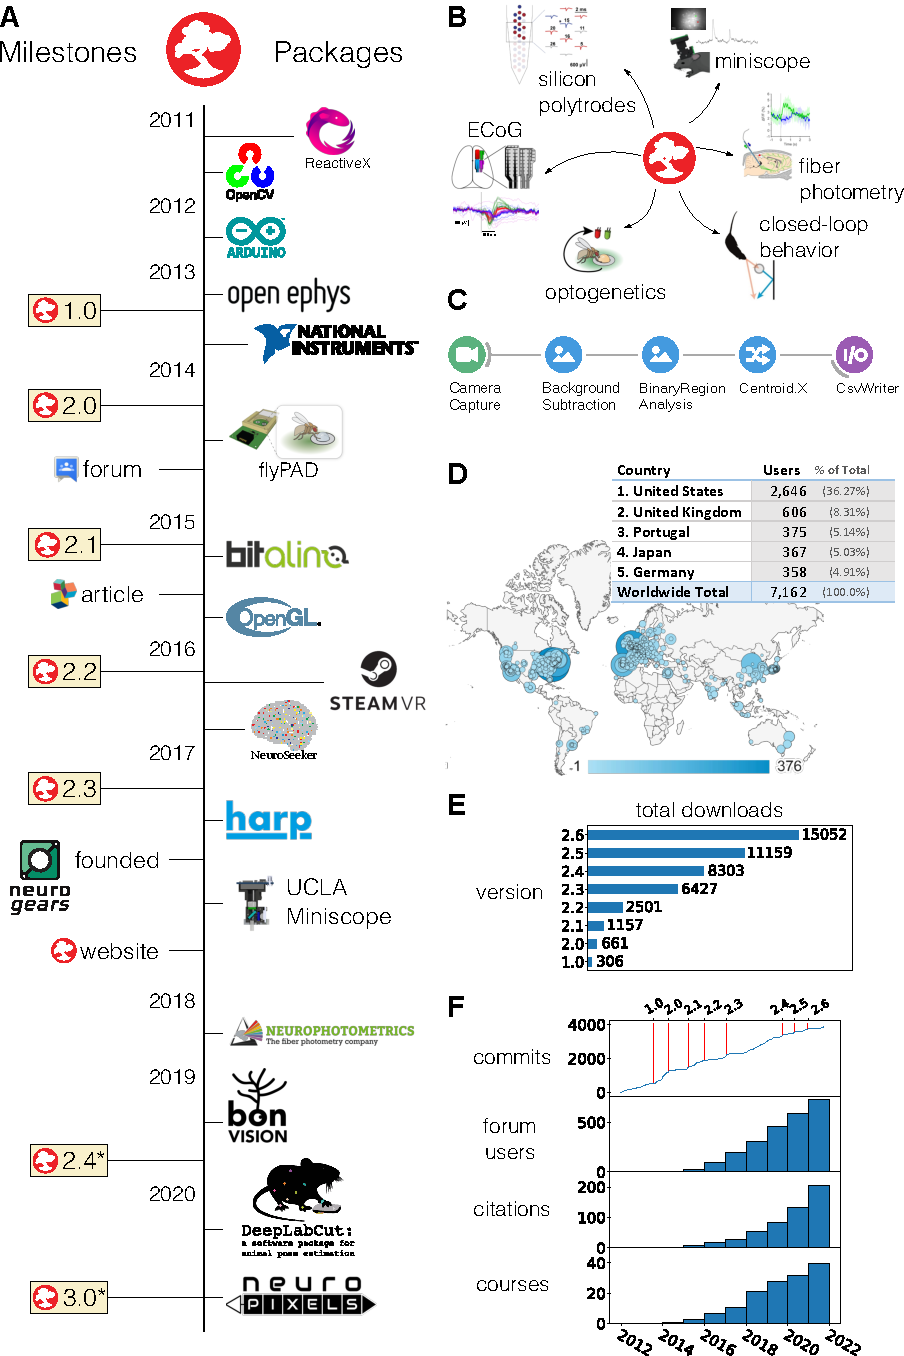
\includegraphics[width=3in]{figures/roadmap-bbsrc-3x.pdf}
	\end{center}
	\caption{Bonsai: development timeline and usage statistics.}
	\label{fig:bonsai}
\end{figure}

Yet, another missing for the implementation of advanced experiments is the
dissemination of expertise in this type of experimentation. This dissemination
is at the core of our proposal.

\subsection{NeuroGEARS-SWC-GCNU collaboration}

NeuroGEARS has been working with the Sainsbury Wellcome Centre and the Gatsby
Computational Neuroscience Unit, both at University College London, for more
than two years developing hardware and software technology for unrestrained,
long-duration, naturalistic, closed-loop and intelligent experimentation in
neuroscience by combining its engineering expertise with the machine learning
and experimental neuroscience research experience of its academic partners.
Together they are opening a new chapter on neuroscience experimentation.

\subsection{Technology dissemination}

The technology that NeuroGEARS is developing in collaboration with the SWC and
the Gatsby Unit is specialised to support neuroscience experiments in rodents.
We offer to generalise this technology to support a wider range of experimental
setups and to distribute it openly to experimentalists around the world.

The potential of disseminating this technology are enormous. Academically,
this technology is allowing to probe systems in natural regimes that cannot
be studied with traditional simpler experiments, and to study these systems in
unprecedented detail. For example in the 24/7 experiments that we
are developing at the SWC we can study foraging in naturalistic environments
where we can control environmental experimental variables (e.g., food delivery)
with great precision, while we record and manipulate neural activity.

The business applications of these technologies are also very large. For
instance in the pharmaceutical industry, these technologies could allow
unprecedented efficiency for automatic drug testing \ldots Another application
appears in the domain of personalised healthcare \ldots

In addition, long-duration, naturalistic and close-loop experiments will
incentivize several adjacent industries, like those of computer storage (to
save the very large amounts of data produced by these experiments), or the
industry of physiological measurement devices (key components in our
experiments).

Furthermore, the novel datasets that our experiments are producing are also
incentivizing academic research in, for example, machine learning algorithms to
process real time time series.

\subsection{Proposal aim}

The current joint work between NeuroGEARS, the SWC and the Gatsby Unit is to
build infrastructure to perform long-duration, naturalistic, close-loop and
intelligent experiments in order to investigate a specifics problems in the
real systems neuroscience. We aim at distributing hardware, software and
machine learning technology to allow a wider range of long-duration,
naturalistic and close-loop experiments.


\section{Core team}
\desc{
List the key members of your team and assign them roles from the following:

\begin{itemize}
    \item project lead (PL)

    \item project co-lead

    \item researcher co-lead (RcL)

    \item specialist

    \item grant manager

    \item professional enabling staff

    \item doctoral student

    \item research and innovation associate

    \item technician

    \item visiting researcher
\end{itemize}

Only list one individual as project lead.
}


\begin{description}
    \item[project lead (PL)]:
    \href{https://neurogears.org/about-us/}{Dr.~Goncalo Lopes}

    \item[researcher co-lead (RcL)]:
        \href{https://www.sainsburywellcome.org/web/people/tiago-branco}{Prof.~Tiago Branco} (SWC),
        \href{https://www.sainsburywellcome.org/web/people/tom-mrsic-flogel}{Prof.~Tom Mrsic-Flogel} (SWC), 
        \href{https://www.gatsby.ucl.ac.uk/~maneesh/}{Prof.~Maneesh Sahani} (GCNU), 

    \item[researcher co-investigator]:
        \href{https://www.sainsburywellcome.org/web/people/dario-campagner}{Dr.~Dario Campagner} (SWC),
        \href{http://www.gatsby.ucl.ac.uk/~rapela/index.html}{Dr.~Joaqu\'{i}n Rapela} (GCNU),

    \item[research fellow]:
        \href{https://www.sainsburywellcome.org/web/people/lorenza-calcaterra-0}{Dr.~Lorenza Calcaterra} (SWC),

    \item[group leader]:
        \href{https://www.sainsburywellcome.org/web/people/jeffrey-erlich}{Dr.~Jeff Erlich} (SWC),

    \item[doctoral student]:
        \href{https://www.sainsburywellcome.org/web/people/jai-bhagat}{Mr.~Jai Bhagat} (SWC),

    \item[undegraduate student]:
        Mrs.~Zimo Li (UCL Neuroscience),

    \item[research assistant]:
        Mrs.~Anaya Pouget (SWC),

    \item[research software engineer]:
        \href{https://neurogears.org/about-us/}{Dr.~Andre Almeida} (NeuroGEARS), 
        \href{https://neurogears.org/about-us/}{Dr.~Andrew Erskine} (NeuroGEARS), 
        \href{https://neurogears.org/about-us/}{Dr.~Jo\~{a}o Fraz\~{a}o} (NeuroGEARS), 
        \href{https://neurogears.org/about-us/}{Dr.~Nicholas Guilbeault} (NeuroGEARS), 
        \href{https://www.sainsburywellcome.org/web/people/chang-huan-lo}{Dr.~Chang Huan Lo} (SWC), 
        \href{https://www.sainsburywellcome.org/web/people/adam-tyson-0}{Dr.~Adam Tyson} (SWC), 
        \href{https://www.sainsburywellcome.org/web/people/niko-sirmpilatze}{Dr.~Niko Sirmpilatze} (SWC), 
        \href{https://www.sainsburywellcome.org/web/people/joe-ziminski}{Dr.~Joe Ziminski} (SWC), 

    \item[research fabrication engineer]:
        \href{https://www.sainsburywellcome.org/web/people/robb-barrett}{Mr.~Rob Barrett} (SWC), 
        \href{https://www.sainsburywellcome.org/web/people/del-halpin}{Mr.~Del Halping} (SWC), 
        \href{https://www.sainsburywellcome.org/web/people/simon-townsend}{Mr.~Simon Townsend} (SWC), 

    \item[research electronics engineer]:
        \href{https://www.sainsburywellcome.org/web/people/graeme-mcphillips}{Mr.~Graeme
        McPhillips} (SWC), 

    \item[grant manager]:
        \href{https://www.ucl.ac.uk/gatsby/people}{Mr.~Mike Sainsbury} (GCNU),

\end{description}



\section{Core questions}

\subsection{Existing relationship}

\desc{
Word limit: 500

What is the existing relationship between the project partners?

\subsubsection*{What the assessors are looking for in your response}

The panel will consider the extent to which the proposed work demonstrates:

\begin{enumerate}

    \item clear evidence of an emerging or established research-based
        relationship between business and academic lead partners with
        demonstrable benefits achieved to date

    \item well considered plans for growing the relationship within and beyond
        the prosperity partnership and a description on where the relationship
        is going long term. The existing relationship will be assessed relative
        to the business lead organisation

    \item ‘substantial’ or ‘long-term’ collaborations and partnerships may look
        different for an or spin-out company than they do for a large
        multinational

\end{enumerate}

}

% \input{existingRelationship}

\subsection{Vision}

\desc{
Word limit: 2,000

What are you hoping to achieve with your proposed work?

\subsubsection*{What the assessors are looking for in your response}

The panel will consider the extent to which the proposed work:

\begin{itemize}

    \item is of excellent quality and importance within or beyond the field(s) or area(s)
    \item has the potential to advance current understanding, or generate new knowledge,
thinking or discovery within or beyond the field or area
is timely given current trends, context, and needs
could impact world-leading research, society, the economy, or the environment
\end{itemize}

Within this section, we expect you to address the following:

\begin{itemize}

    \item a clear and appropriate business-led vision and ambition for the
        prosperity partnership describing why the partnership is essential for
        success and specifically addressing why the objectives cannot be
        achieved by any single partner alone

    \item evidence that the proposed business-led research programme is
        positioned at technology readiness levels (TRL) one to four with a
        programme of work that has been developed in partnership and in a
        co-created manner with the short-term and medium-term benefits clearly
        described

    \item coherence and relevance of the work packages in line with the vision

    \item clear evidence of how this vision will be achieved and how the
        prosperity partnership will bring benefits to the UK economy and the
        research base, address regional, national, and international
        strategies, including those of the business or businesses involved

\end{itemize}

Within this section you can demonstrate elements of your responses in visual
form if relevant. Further instructions are provided within the Funding Service.

Number your references in this section using a superscript citation style. Then
include the details of these references in a corresponding list, in the
‘References’ section of this application.

Please note, external weblinks are not permitted in this section.
}

% \input{vision}

\subsection{Additionality and added value}

\desc{
Word limit: 300

\subsubsection*{What is the additionality and added value?}

What the assessors are looking for in your response

The panel will consider the extent to which the proposed work demonstrates:

\begin{itemize}

    \item evidence of the additionality and added value of a prosperity
        partnership in

    \item comparison to other funding opportunities

    \item clear evidence of the buy-in from business partners and co-creation
        of the proposed business-inspired fundamental research programme

\end{itemize}

Within this section, we expect you to consider:

\begin{itemize}

    \item the aspects where this type of funding provides added value that no
        other scheme does

\end{itemize}

}

% \input{additionality}

\subsection{Applicants’ leadership and appropriateness of the team}

\desc{
Word limit: 300

\subsubsection*{What are your leadership and team track records?}

What the assessors are looking for in your response

The panel will consider the extent to which the proposed work demonstrates:

\begin{itemize}

    \item the appropriateness of the leadership team with evidence of joint
        working between business and the academic project lead

    \item clear plans for joint leadership conveying the ability to lead a
        programme of this size and number of stakeholders

    \item how you approached the design and makeup of the team’s skills and
        competencies in order to address the vision and ambition of the
        programme

\end{itemize}

Within this section, we expect you to consider:

\begin{itemize}

    \item your track record in successfully leading large multifaceted teams that involve
cross organisational complexity

    \item explain why you think you have the most appropriate balance of expertise

    \item your ability to lead a programme of this size and number of stakeholders
\end{itemize}

}

% \input{leadership}

\subsection{Management and governance}

\desc{
Word limit: 300

\subsection*{What are your plans for management and governance?}

What the assessors are looking for in your response

The panel will consider the extent to which the proposed work demonstrates:

\begin{itemize}

    \item the appropriateness of the management and governance arrangements,
commensurate with the scale of the programme

    \item how you will monitor milestones and ensure they are achieved

    \item your plans regarding equality, diversity and inclusion that go beyond following
university procedures

\end{itemize}

}

% \input{management}

\subsection{Impact}

\desc{
Word limit: 300

\subsection*{How will you deliver impact and ensure benefits are realised?}

What the assessors are looking for in your response

The panel will consider the extent to which the proposed work demonstrates:

\begin{itemize}

    \item how the prosperity partnership will deliver the benefits identified
    \item clear plans to maximise translation and impact arising from the partnership

\end{itemize}

Within this section, we expect you to consider:

\begin{itemize}

    \item the potential direct or indirect

    \item benefits and who the beneficiaries might be

\end{itemize}

}

% \input{impact}

\subsection{Skills and talent training}

\desc{
Word limit: 300

\subsection*{What are your plans and requirements for workforce training and development in
support of the strategic objectives of the proposed prosperity partnership?}

What the assessors are looking for in your response

The panel will consider the extent to which the proposed work demonstrates:

\begin{itemize}

    \item that an excellent and inclusive training environment will be provided
        which is appropriate for alignment with the prosperity partnership

    \item how the skills being developed will enable the delivery of the
        prosperity partnership’s goals and that the delivery of the plan is
        feasible

    \item how the plan will offer career development opportunities for the
        people in receipt of this training

\end{itemize}

Within this section, we expect you to consider:

\begin{itemize}

    \item how the whole project team, from both the research organisation and
        the business, will receive appropriate training and research experience

\end{itemize}

}

% \input{skillsAndTalentsTraining}

\subsection{Ethics and responsible research and innovation (RRI)}

\desc{
Word limit: 300

What are the ethical or RRI implications and issues relating to the proposed
work? If you do not think that the proposed work raises any ethical or RRI
issues, explain why.

What the assessors are looking for in your response

The panel will consider the extent to which the proposed work demonstrates that
you have identified and evaluated:

\begin{itemize}

    \item the relevant ethical or responsible research and innovation consideration

    \item show you will manage these considerations

\end{itemize}
}

% \input{responsibleResearchAndInnovation}

\subsection{Resources}

\desc{
Word limit: 400

In this section we will ask for the following:

\begin{itemize}

    \item what is the full economic cost of your project?

    \item what is the total value of funding being requested from BBSRC?

    \item what is the total value of the business lead’s cash contribution?

    \item what is or are the individual cash contributions of additional project partners?

    \item what is the total value of the project lead’s organisation’s cash contribution?

    \item what is the total project value?

    \item what is the total value of the business lead’s in-kind contributions?

    \item what is the total value of the project lead’s organisation’s in-kind contributions?

    \item what is the total value of the additional project partners (academic and business) in-kind contributions?

    \item what is the overall project value?

\end{itemize}

In the Funding Service a table will be provided that can be used to complete
your response.

What the assessors are looking for in your response

We are looking for a resources budget which sets out the request for BBSRC
funding and the appropriate business and academic cash and in-kind
contributions
to the programme.

Specific details of the matched contributions may not be available at this
stage.  Therefore, a 10\% variation, in addition to a shift in the breakdown
across headings is accepted in the total of the project value from the outline
stage and the full proposal stage. All contributions will be validated again at
full proposal stage.

}

% \input{resources}

\subsection{Your organisation’s support}

\desc{
Word limit: 5

Provide details of support from your research organisation.

What the assessors are looking for in your response

Provide a Statement of Support from your research organisation detailing why
the proposed work is needed. This should include details of any funding that
will be provided to support the activity and any additional support that might
add value to the work.

The committee will be looking for a strong statement of commitment from your
research organisation.

We recognise that in some instances, this information may be provided by your
Head of Department of School, the Research Office, the Technology Transfer
Office (TTO) or equivalent, or a combination.

You must also include the following details:

\begin{itemize}

    \item a significant person’s name and their position, from your organisation’s Head of
Department or School, the TTO or Research Office, or a combination

    \item office address or web link

\end{itemize}

Upload details are provided within the service on the actual application.

}

\subsection{Project partners}

\desc{
Word limit: 5

Provide details of any project partners’ contributions, and letters or emails
of support from the business(es) involved.

Each letter or email you provide should:

\begin{itemize}

    \item the name and the company number of the business

    \item details of the cash and in-kind contributions from the business

    \item have a confirmation statement from the business lead that they will
        be leading the project, dated, and signed by a relevant representative
        from the business

    \item highlight conflicts or information we should be aware of despite us
        not expecting confidential information at this stage

\end{itemize}

Save letters or emails of support from each partner in a single PDF no bigger
than 8MB. Unless specially requested, please do not include any personal data
within the attachment.

The Funding Service will provide document upload details when you apply.
}

\subsection{References}

\desc{
Word limit: 1,000

List the references you have used to support your application.

What the assessors are looking for in your response

\begin{itemize}

    \item include all references in this section, not in the rest of the
        application questions

    \item you should not include any other information in this section

    \item we advise you not to include hyperlinks, as assessors are not obliged
        to access the information they lead to or consider it in their
        assessment of your application

    \item if linking to web resources, to maintain the information’s integrity,
        include persistent identifiers (such as digital object identifiers)
        where possible

    \item you must not include links to web resources to extend your
        application

\end{itemize}
}

\end{document}
